\documentclass[12pt,a4paper]{article}

\usepackage[utf8]{inputenc}
\usepackage{amsmath}
\usepackage{graphicx}


\usepackage{makeidx}
\newcommand{\RuntimeHead}{Runtime}
\newcommand{\AdvantageHead}{Advantage}
\newcommand{\DisadvantageHead}{Disadvantage}
\newcommand{\ImplementationInJavaHead}{Implementation in Java}
\newcommand{\TypicalAlgorithmHead}{Typical Algorithm}

\begin{document}
\tableofcontents
\newpage

\section{Data Structures}
Access means that your are given the index and you have to return the element on this index.
Search means, that your are given an element and you to find it in an Data Structure. 
Deletion means, that the element is deleted from the Data Structure.
\subsection{Arrays}
An array is a container object that holds a fixed number of values of a single type. The length of an array is established when the array is created. After creation, its length is fixed. Y
\subsubsection{\RuntimeHead}
Average: 
Access: $\theta(1)  $
Search: $\theta(n) $
Insertion: $ \theta(n)$
Deletion: $\theta (n)$
\newline
\newline
Worst Case: 
Access: $O(1)$  
Search: $O(n) $
Insertion: $O(n)$
Deletion: $O(n)$
\newline
\newline
Deletion is in $O(n)$, because we  have to copy the rest of the array to a new array. Or in an unsorted array, we swap the element to the end of the array and decrease the size of the array by one. 


\subsubsection{\AdvantageHead}
\begin{itemize}
\item Fast Acces.
\item It is used to represent multiple data items of same type by using only single name.
\item More dimensional Data Structure.
\item Less memory footprints than i.e. a List, because no Pointer to the next/previos element needed (in Java).
\end{itemize}
\subsubsection{\DisadvantageHead}
\begin{itemize}
\item We must know in advance that how many elements are to be stored in array.
\item Waste of memory, if more space allocated than needed.
\item The elements of array are stored in consecutive memory locations. So insertions and deletions are very difficult and time consuming.
\end{itemize}
\subsubsection{\ImplementationInJavaHead}
java.util.Arrays provides useful methods for arrays such as binarySearch or sort.

\subsubsection{\TypicalAlgorithmHead}
Used for Matrices and Vectors.

\subsection{ArrayList}
Resizable-array implementation of the List interface. Implements all optional list operations, and permits all elements, including null. In addition to implementing the List interface, this class provides methods to manipulate the size of the array that is used internally to store the list. (This class is roughly equivalent to Vector, except that it is unsynchronized.) 	
\subsubsection{\RuntimeHead}
Average: 
Access: $\theta(1)  $
Search: $\theta(n) $
Insertion: $ \theta(1)$ if the element is inserted at the end of the array
Deletion: $\theta (n)$
\newline
\newline
Worst Case: 
Access: $O(1)$  
Search: $O(n) $
Insertion: $O(1)$ if the element is inserted at the end of the array
Deletion: $O(n)$


\subsubsection{\AdvantageHead}
\begin{itemize}
\item variable length
\item Fast access
\item Insertion in average in $\theta(1)$
\end{itemize}
\subsubsection{\DisadvantageHead}
\begin{itemize}
\item Insertion may cause copying of the ArrayList.
\item Fast access.
\item Insertion in average in $\theta(1)$. Insertion/Deletion may cause copying of the ArrayList.
\end{itemize}
\subsubsection{\ImplementationInJavaHead}
java.util.ArrayList
\subsubsection{\TypicalAlgorithmHead}

\subsection{Single LinkedList}

\subsubsection{\RuntimeHead}
Average: 
Access: $\theta(n)  $
Search: $\theta(n) $
Insertion: $ \theta(1)$ if the element is inserted at the end of the array or a pointer to the previous element is given.
Deletion: $\theta (n)$ if last element is deleted or a pointer to the element is given.

Worst Case: 
Access: $O(n)$  
Search: $O(n) $
Insertion: $O(1)$ if the element is inserted at the end of the array or a pointer to the previous element is given.
Deletion: $O(1)$ if the last element is deleted or a pointer to the element is given.
\subsubsection{\AdvantageHead}
\begin{itemize}
\item No limited size (except for the available memory)
\item Fast insertion. 
\item No memory waste (except for pointers to the next element)
\end{itemize}
\subsubsection{\DisadvantageHead}
\begin{itemize}
\item Slow Access to elements. (i.e. no binary Search possible)
\item Another advantage of arrays in access time is special locality in memory. Arrays are defined as contiguous blocks of memory, and so any element will be physically near its neighbours.This greatly benifits from modern CPU caching methods.
\item Extra memory for a pointer is required.
\end{itemize}
\subsubsection{\ImplementationInJavaHead}
java.util.LinkedList
\subsubsection{\TypicalAlgorithmHead}

\subsection{Double LinkedList}
Nearly the same as Single Linked List. But every element holds a pointer to the previos element. So backward traversion is possible and more memory is needed.

\subsection{Stack}
In computer science, a stack is an abstract data type that serves as a collection of elements, with two principal operations: push, which adds an element to the collection, and pop, which removes the most recently added element that was not yet removed. The order in which elements come off a stack gives rise to its alternative name, LIFO (for last in, first out). Additionally, a peek operation may give access to the top without modifying the stack.
\subsubsection{\RuntimeHead}
Average: 
Access: $\theta(n)  $
Search: $\theta(n) $
Insertion: $ \theta(1)$ 
Deletion: $\theta (n)$ 

Worst Case: 
Access: $O(n)$  
Search: $O(n) $
Insertion: $O(1)$ 
Deletion: $O(1)$ 

\subsubsection{\AdvantageHead}
\begin{itemize}
\item No limited size (except for the available memory)
\item Fast insertion. 
\item No memory waste
\end{itemize}
\subsubsection{\DisadvantageHead}
\begin{itemize}
\item Slow Access to elements. (i.e. no binary Search possible)
\end{itemize}
\subsubsection{\ImplementationInJavaHead}
java.util.Stack \\
public class $Stack<E>$
extends $Vector<E>$
\subsubsection{\TypicalAlgorithmHead}
\begin{itemize}
\item Polish Notation
\item Backtracking
\item Java Virtual Machine
\end{itemize}



\subsection{Queue}
In computer science, a queue is a particular kind of abstract data type or collection in which the entities in the collection are kept in order and the principal (or only) operations on the collection are the addition of entities to the rear terminal position, known as enqueue, and removal of entities from the front terminal position, known as dequeue. This makes the queue a First-In-First-Out (FIFO) data structure. In a FIFO data structure, the first element added to the queue will be the first one to be removed.
\subsubsection{\RuntimeHead}
Average: 
Access: $\theta(n)  $
Search: $\theta(n) $
Insertion: $ \theta(1)$ 
Deletion: $\theta (n)$ 

Worst Case: 
Access: $O(n)$  
Search: $O(n) $
Insertion: $O(1)$ 
Deletion: $O(1)$ 

\subsubsection{\AdvantageHead}
\begin{itemize}
\item No limited size (except for the available memory)
\item Fast insertion. 
\item No memory waste
\end{itemize}
\subsubsection{\DisadvantageHead}
\begin{itemize}
\item Slow Access to elements. (i.e. no binary Search possible)
\end{itemize}
\subsubsection{\ImplementationInJavaHead}
Interface $Queue<E>$ java.util 
All Known Implementing Classes:\\
AbstractQueue, ArrayBlockingQueue, ArrayDeque, ConcurrentLinkedQueue, DelayQueue, LinkedBlockingDeque, LinkedBlockingQueue, LinkedList, PriorityBlockingQueue, PriorityQueue, SynchronousQueue
\subsubsection{\TypicalAlgorithmHead}


\subsection{PriorityQueue}
In computer science, a priority queue is an abstract data type which is like a regular queue or stack data structure, but where additionally each element has a "priority" associated with it. In a priority queue, an element with high priority is served before an element with low priority. If two elements have the same priority, they are served according to their order in the queue.\\
Note: Implementation is often done with heaps, a data structure that uses arrays (fixed size or dynamic array). java.util.PriorityQueue uses also an array, that grows by 50 percent for huge arrays, 100 percent for small arrays)
\subsubsection{\RuntimeHead}
Binary PriorityQueue:\\
Average: 
Access: $\theta(log n)  $
Search: $\theta(log n) $
Insertion: $ \theta(log n)$ 
Deletion of min element: $\theta (log n)$ 

Worst Case: 
Access: $O(log n)$  
Search: $O(log n) $
Insertion: $O(log n)$ 
Deletion of min element: $O(log n)$ 
\\
\newline
Fibonacci PriorityQueue:\\
Average: 
Access: $\theta(log n)  $
Search: $\theta(log n) $
Insertion: $ \theta(1)$ 
Deletion of min element: $\theta (log n)$ 

Worst Case: 
Access: $O(log n)$  
Search: $O(log n) $
Insertion: $O(1)$ 
Deletion of min element: $O(log n)$ 
\newline

Fibonacci Heap is faster in InsertMin $\theta (1)$ and in decrease-key $\theta (1)$ versus$O(log n)$ for Binary Priority Queue.  	

\subsubsection{\AdvantageHead}
\begin{itemize}
\item Elements are sorted
\item Inserting new elements is faster than in an sorted array or sorted List
\item Sorting takes time $\theta (n)$ with a fibonacci Priority Queue.
\end{itemize}
\subsubsection{\DisadvantageHead}
\begin{itemize}
\item Slower Insertion, Deletion, Access
\end{itemize}
\subsubsection{\ImplementationInJavaHead}
java.util.PriorityQueue (Implementation note: this implementation provides O(log(n)) time for the enqueing and dequeing methods (offer, poll, remove() and add); linear time for the remove(Object) and contains(Object) methods; and constant time for the retrieval methods (peek, element, and size). )
\subsubsection{\TypicalAlgorithmHead}
\begin{itemize}
\item Dijkstra's algorithm
\item Best-first search algorithms
\item Prim's algorithm for minimum spanning tree
\item Bandwidth management
\end{itemize}

\subsection{SkipList}
SkipList is a ordered list.\\
A skip list is built in layers. The bottom layer is an ordinary ordered linked list. Each higher layer acts as an "express lane" for the lists below, where an element in layer i appears in layer i+1 with some fixed probability p (two commonly used values for p are $\frac{1}{2}$ or $\frac{1}{4}$). On average, each element appears in $\frac{1}{1-p}$ lists, and the tallest element (usually a special head element at the front of the skip list) in all the lists. The skip list contains $log_{1/p}n$ lists.

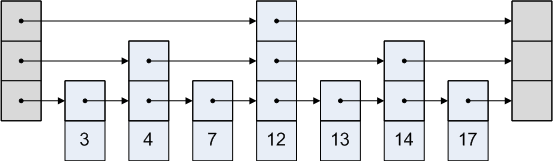
\includegraphics[]{SkipList}
Decide how many lists will a node be part of. With probabily of $\frac{1}{2}$ node will be part of the lowest level only, with $\frac{1}{4}$ node will be part of the two lowest list and so on.\\
See http://igoro.com/archive/skip-lists-are-fascinating/ for more details.


\subsubsection{\RuntimeHead}
Average: 
Access: $\theta(log n)  $
Search: $\theta(log n) $
Insertion: $ \theta(log n)$ 
Deletion: $\theta (log n)$ 

Worst Case: 
Access: $O( n)$  
Search: $O( n) $
Insertion: $O(n)$ 
Deletion: $O( n)$ 
\newline
\subsubsection{\AdvantageHead}
\begin{itemize}
\item Faster search and insertion of elements (as fast as balanced AVL-Trees)
\item Elements are sorted
\item Easy to implement
\end{itemize}
\subsubsection{\DisadvantageHead}
\begin{itemize}
\item Space Complexity $O(n*log(n))$
\end{itemize}
\subsubsection{\ImplementationInJavaHead}
There is no implementation in java. But java.util.concurrent.ConcurrentSkipListSet<E> and java.util.concurrent.ConcurrentSkipListMap<K,V> are using the same logic.
\subsubsection{\TypicalAlgorithmHead}

\subsection{HashTable}
In computing, a hash table (hash map) is a data structure used to implement an associative array, a structure that can map keys to values. A hash table uses a hash function to compute an index into an array of buckets or slots, from which the desired value can be found.

Ideally, the hash function will assign each key to a unique bucket, but most hash table designs employ an imperfect hash function, which might cause hash collisions where the hash function generates the same index for more than one key. Such collisions must be accommodated in some way.
\subsubsection{\RuntimeHead}
Average: 
Access: N/A\\
Search: $\theta(1) $
Insertion: $ \theta(1)$ 
Deletion $\theta (1)$ 

Worst Case: 
Access:  N/A\\
Search: $O( n) $
Insertion: $O(n)$ 
Deletion of min element: $O(n)$ 
\subsubsection{\AdvantageHead}
\begin{itemize}
\item Fast operations
\item If the number of entries can predicted in advance, it is particulary efficient (no need to resize buckets)
\end{itemize}
\subsubsection{\DisadvantageHead}
\begin{itemize}
\item Cost of a good hash function can slow the programm (if number of entries is small)
\item Not ordered
\item Slow for applications like spell-checking
\item Dynammic Resizing of the hash table
\item Poor locality of reference, data  to be accessed is distributed seemingly at random in memory
\item Inefficient when there are many collisions
\end{itemize}
\subsubsection{\ImplementationInJavaHead}
java.util.HashSet<E> (Implemantation in java uses an array that contains Entry. Entry has an pointer to its next element)\\
java.util.HashMap<K,V>\\
LinkedHashSet<E> (Hash table and linked list implementation of the Set interface. An insertion-ordered Set implementation that runs nearly as fast as HashSet.)\\
java.util.LinkedHashMap<K,V> (Hash table and linked list implementation of the Map interface. An insertion-ordered Map implementation that runs nearly as fast as HashMap. Also useful for building caches (see removeEldestEntry(Map.Entry) )).\\
java.util.WeakHashMap<K,V> ( An implementation of the Map interface that stores only weak references to its keys. Storing only weak references allows key-value pairs to be garbage-collected when the key is no longer referenced outside of the WeakHashMap. This class provides the easiest way to harness the power of weak references. It is useful for implementing "registry-like" data structures, where the utility of an entry vanishes when its key is no longer reachable by any thread.)\\
ConcurrentHashMap  (A highly concurrent, high-performance ConcurrentMap implementation based on a hash table. This implementation never blocks when performing retrievals and allows the client to select the concurrency level for updates. It is intended as a drop-in replacement for Hashtable: in addition to implementing ConcurrentMap, it supports all of the "legacy" methods peculiar to Hashtable.)
\subsubsection{\TypicalAlgorithmHead}

\subsection{Binary Search Tree}
A binary search tree is a rooted binary tree, whose internal nodes each store a key (and optionally, an associated value) and each have two distinguished sub-trees, commonly denoted left and right. The tree additionally satisfies the binary search tree property, which states that the key in each node must be greater than all keys stored in the left sub-tree, and not greater than any key in the right sub-tree.[1]:287 (The leaves (final nodes) of the tree contain no key and have no structure to distinguish them from one another. Leaves are commonly represented by a special leaf or nil symbol, a NULL pointer, etc.)
\subsubsection{\RuntimeHead}
This chapter examines basic Binary Search Trees (that are not full)\\
Average: 
Access: $\theta(log n)  $
Search: $\theta(log n)  $
Insertion: $\theta(log n)  $
Deletion $\theta(log n)  $\\
Average means, that the inserted elements are sorted randomly. If they are sorted in decreasing Order all this operations take $O(n)$ time.x

Worst Case: 
Access:  $O(n)$ 
Search: $O(n) $
Insertion: $O(n)$ 
Deletion: $O(n)$ 
\subsubsection{\AdvantageHead}
\begin{itemize}
\item Sorting and Search can be very fast.
\item Easy to implement.
\item Useful for other data structure like Priority Queues.
\end{itemize}
\subsubsection{\DisadvantageHead}
\begin{itemize}
\item Can be slow if order of elements is not randomly.
\end{itemize}
\subsubsection{\ImplementationInJavaHead}
There exists no implementation of basic Binary Search Tree in Java api.
\subsubsection{\TypicalAlgorithmHead}
Search and Sort.

\subsection{Cartesian Tree}
A Cartesian tree is a tree data structure created from a set of data that obeys the  following structural invariants:
\begin{itemize}
\item The tree obeys in the min (or max) heap property – each node is less (or greater) than its children.
\item An inorder traversal of the nodes yields the values in the same order in which they appear in the initial sequence.
\end{itemize}

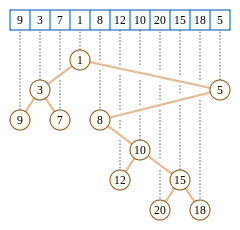
\includegraphics[]{CartesianTree}
\subsubsection{\RuntimeHead}
Average: 
Access: N/A \\
Search: $\theta(log n)  $
Insertion: $\theta(log n)  $
Deletion $\theta(log n)  $\\
Average means, that the inserted elements are sorted randomly. If they are sorted in decreasing Order all this operations take $O(n)$ time.x

Worst Case: 
Access:  N/A \\
Search: $O(n) $
Insertion: $O(n)$ 
Deletion: $O(n)$ 
\subsubsection{\AdvantageHead}
\begin{itemize}
\item Elements are sorted like they were inserted
\item Min value between to node is fast to determine
\end{itemize}
\subsubsection{\DisadvantageHead}
\begin{itemize}
\item No Access to a specific element.
\end{itemize}
\subsubsection{\ImplementationInJavaHead}
\subsubsection{\TypicalAlgorithmHead}
\begin{itemize}
\item Cartesian Tree Sorting
\item Used for Treap data structure
\end{itemize}

\subsection{B-Tree}
nochhmal durchlesen, sehr interessant im Algorithms Buch
\subsubsection{\RuntimeHead}
\subsubsection{\AdvantageHead}
\subsubsection{\DisadvantageHead}
\subsubsection{\ImplementationInJavaHead}
\subsubsection{\TypicalAlgorithmHead}

\subsection{Red-Black-Tree}
A red–black tree is a kind of self-balancing binary search tree. Each node of the binary tree has an extra bit, and that bit is often interpreted as the color (red or black) of the node. These color bits are used to ensure the tree remains approximately balanced during insertions and deletions. There are 5 properties that must be satisfied by a Red-Black-Tree:\\

\begin{itemize}
\item Each node is either red or black.
\item The root is black. This rule is sometimes omitted. Since the root can always be changed from red to black, but not necessarily vice versa, this rule has little effect on analysis.
\item All leaves (NIL) are black.
\item If a node is red, then both its children are black.
\item Every path from a given node to any of its descendant NIL nodes contains the same number of black nodes. Some definitions: the number of black nodes from the root to a node is the node's black depth; the uniform number of black nodes in all paths from root to the leaves is called the black-height of the red–black tree.
\end{itemize}

No path from the root to a leaf is more than twice as long as any other path from the root to a leaf.\\

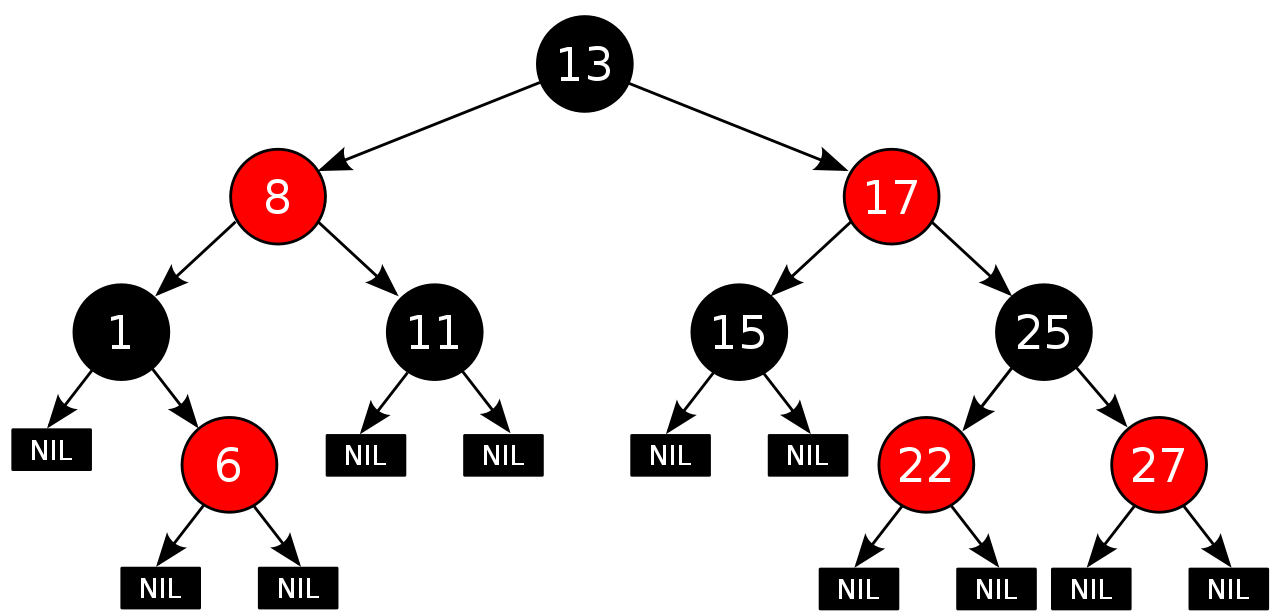
\includegraphics[scale=0.3]{RedBlackTree}
\subsubsection{\RuntimeHead}
Average: 
Access: $O(log n) $
Search: $O(log n) $
Insertion: $O(log n) $
Deletion $O(log n) $\\
Average means, that the inserted elements are sorted randomly. If they are sorted in decreasing Order all this operations take $O(n)$ time.x

Worst Case: 
Access: $O(log n) $
Search: $O(log n) $
Insertion: $O(log n) $
Deletion: $O(log n) $ 
\subsubsection{\AdvantageHead}
\begin{itemize}
\item Faster Worst Case Operations than on a binary Tree.
\item Sorting and Search can be fast.
\item Particularly useful when inserts and/or deletes are relatively frequent.
\end{itemize}
\subsubsection{\DisadvantageHead}
\begin{itemize}
\item Complicated to implement.
\item If you plan to only build the tree once and then only perform read operations thereafter, AVL trees offer better performance. (In practice, this performance gain is usually negligible,
\item B-Trees are prefered for storing a large amount of information on disk.
\end{itemize}
\subsubsection{\ImplementationInJavaHead}
java.util.TreeSet and java.util.TreeMap
\subsubsection{\TypicalAlgorithmHead}
\begin{itemize}
\item Many data structures used in computational geometry can be based on red–black trees.
\item The Completely Fair Scheduler used in current Linux kernels uses red–black trees.
\item In the version 8 of Java, the Collection HashMap has been modified such that instead of using a LinkedList to store different elements with identical hashcodes, a Red-Black tree is used.
\end{itemize}
\subsection{Splay-Tree}
\subsubsection{\RuntimeHead}
\subsubsection{\AdvantageHead}
\subsubsection{\DisadvantageHead}
\subsubsection{\ImplementationInJavaHead}
\subsubsection{\TypicalAlgorithmHead}

\subsection{AVL-Tree}
\subsubsection{\RuntimeHead}
\subsubsection{\AdvantageHead}
\subsubsection{\DisadvantageHead}
\subsubsection{\ImplementationInJavaHead}
\subsubsection{\TypicalAlgorithmHead}

\subsection{KD-Tree}
\subsubsection{\RuntimeHead}
\subsubsection{\AdvantageHead}
\subsubsection{\DisadvantageHead}
\subsubsection{\ImplementationInJavaHead}
\subsubsection{\TypicalAlgorithmHead}
\end{document}

